\section{La sécurité des transports en commun}
    \subsection{Un contexte mondial}
        Le bon fonctionnement des transports en commun dépend de nombreux facteurs. Qu'il soit humain, ou bien technique, le moindre dysfonctionnement impactera le système entier très rapidement. Ainsi, un simple tour d'horizon de la presse internationale fait vite remonter à la surface de nombreux cas de paralysie des transports publics urbains dans le monde entier.

        \subsubsection{Les risques d'atteinte aux passagers}
            Parmi tous les cas de paralysie, les plus marquants à l'échelle internationale sont ceux impliquant des dégâts humains importants parmi les passagers. Il s'agit, dans la plupart des cas, d'attaques terroristes. Bien qu'ils soient relativement rares, le lourd bilan humain de ces attentats marque durablement les esprits.

            C'est le cas de l'attentat à la bombe dans la gare Saint-Michel du train inter-urbain parisien, le 25 juillet 1995, qui provoqua la mort de 8 personnes~\cite{stmichel}. L'attaque la plus marquante de l'histoire fut celle du 7 juillet 2005 dans la ville de Londres. Quatre attentats-suicides dans différentes rames de métro provoquent la mort de 56 personnes et en blessent 700 autres~\cite{london_attacks}.

        \subsubsection{Le risque des mouvements sociaux}
            Si ces attaques sont impressionnantes et marquantes pour la population, elles restent minoritaires dans les cas de paralysie. Parmi les cas de paralysie que nous avons recensé, nous pouvons constater que la majorité des cas de blocage des transports en commun sont provoqués par le personnel des compagnies gérant ces transports. En effet, lors de conflits sociaux, le personnel possède un énorme moyen de pression sur la hiérarchie car il peut bloquer l'intégralité du trafic en se mettant en grève. 

            C'est le cas à Londres, où un plan de fermeture des guichets du métro a provoqué une grève massive le 28 avril 2014. Cela a entraîné la fermeture des deux tiers des stations et la diminution du trafic de 50\%~\cite{tubeApril}. Mais aussi à San Francisco, en juillet et octobre 2013, où une grève du réseau ferré interurbain (forte de ses quatre-cent-mille passagers par jour) a paralysé la ville pendant plusieurs jours~\cite{SFbart}.

    \subsection{La situation en France}
        En France, il arrive aussi que les réseaux de transports en commun soient mis en difficulté. Les archives ne contiennent peu de traces de graves attentats tels que cités précédemment : la plupart du temps, les troubles sont dus à des grèves du personnel pouvant refléter différentes réclamations.
        
        \subsubsection{Les évènements notables dans tout le pays}
            Commençons par Marseille en décembre 2013, où les conducteurs ont réussi à bloquer la quasi-totalité du réseau pendant plus de deux jours. Ils protestaient contre les salaires, la pénibilité en fin de carrière et la suppression de deux jours de congés. Cela est également arrivé à Lille en mai 2014, où le tramway et les bus ont été immobilisés par les traminots demandant une hausse des salaires.

            Mais parfois, les grèves sont la conséquence de certains incidents survenus lors des trajets. Le plus souvent, il s'agit d'agressions sur le personnel, qui sont plus fréquentes qu'on ne pourrait le penser.

            À Dunkerque en mai 2013 par exemple, un chauffeur subit une agression de la part de voyageurs, qui l'ont poursuivi en voiture jusqu'au terminus de la ligne. Arrivés là, équipés d'extincteurs, ils ont bloqué le bus et menacé ses occupants. La Confédération Générale du Travail (CGT) a été avertie, une plainte a été déposée et les conducteurs ont exercé leur droit de retrait, paralysant ainsi le réseau pendant toute une journée.

            C'est ensuite à Douai, en septembre de la même année, que trois contrôleurs sont agressés lors d'un contrôle par une vingtaine de personnes. Des coups sont échangés, les trois hommes finissent à l'hôpital avec des contusions et une entorse au poignet pour l'un d'entre eux. L'ensemble des contrôleurs du réseau exerce alors son droit de retrait, bloquant celui-ci pendant une journée entière.

            Mais qu'en est-il au sein de l'agglomération rennaise, qui nous intéresse tout particulièrement dans le cadre de ce projet ? Tout d'abord, décrivons le réseau de transports actuellement en place, ainsi que sa gestion.
                
        \subsubsection{Le cas rennais}
            Le réseau de transports rennais est constitué d'une ligne de métro (une deuxième étant en construction) et d'un réseau de bus. Ces deux éléments sont gérés par le Service des Transports en commun de l'Agglomération Rennaise (STAR), qui dépend de la société Keolis Rennes. Le STAR a également mis en place depuis quelques années un système de vélos en libre-service : les vélos STAR. Les usagers peuvent accéder aux différents services du STAR par plusieurs moyens : en achetant des tickets à l'unité (pour bus et métro), ou en utilisant une carte d'abonné rechargeable (la carte Korrigo). 

            \begin{figure}
                \begin{center}
                    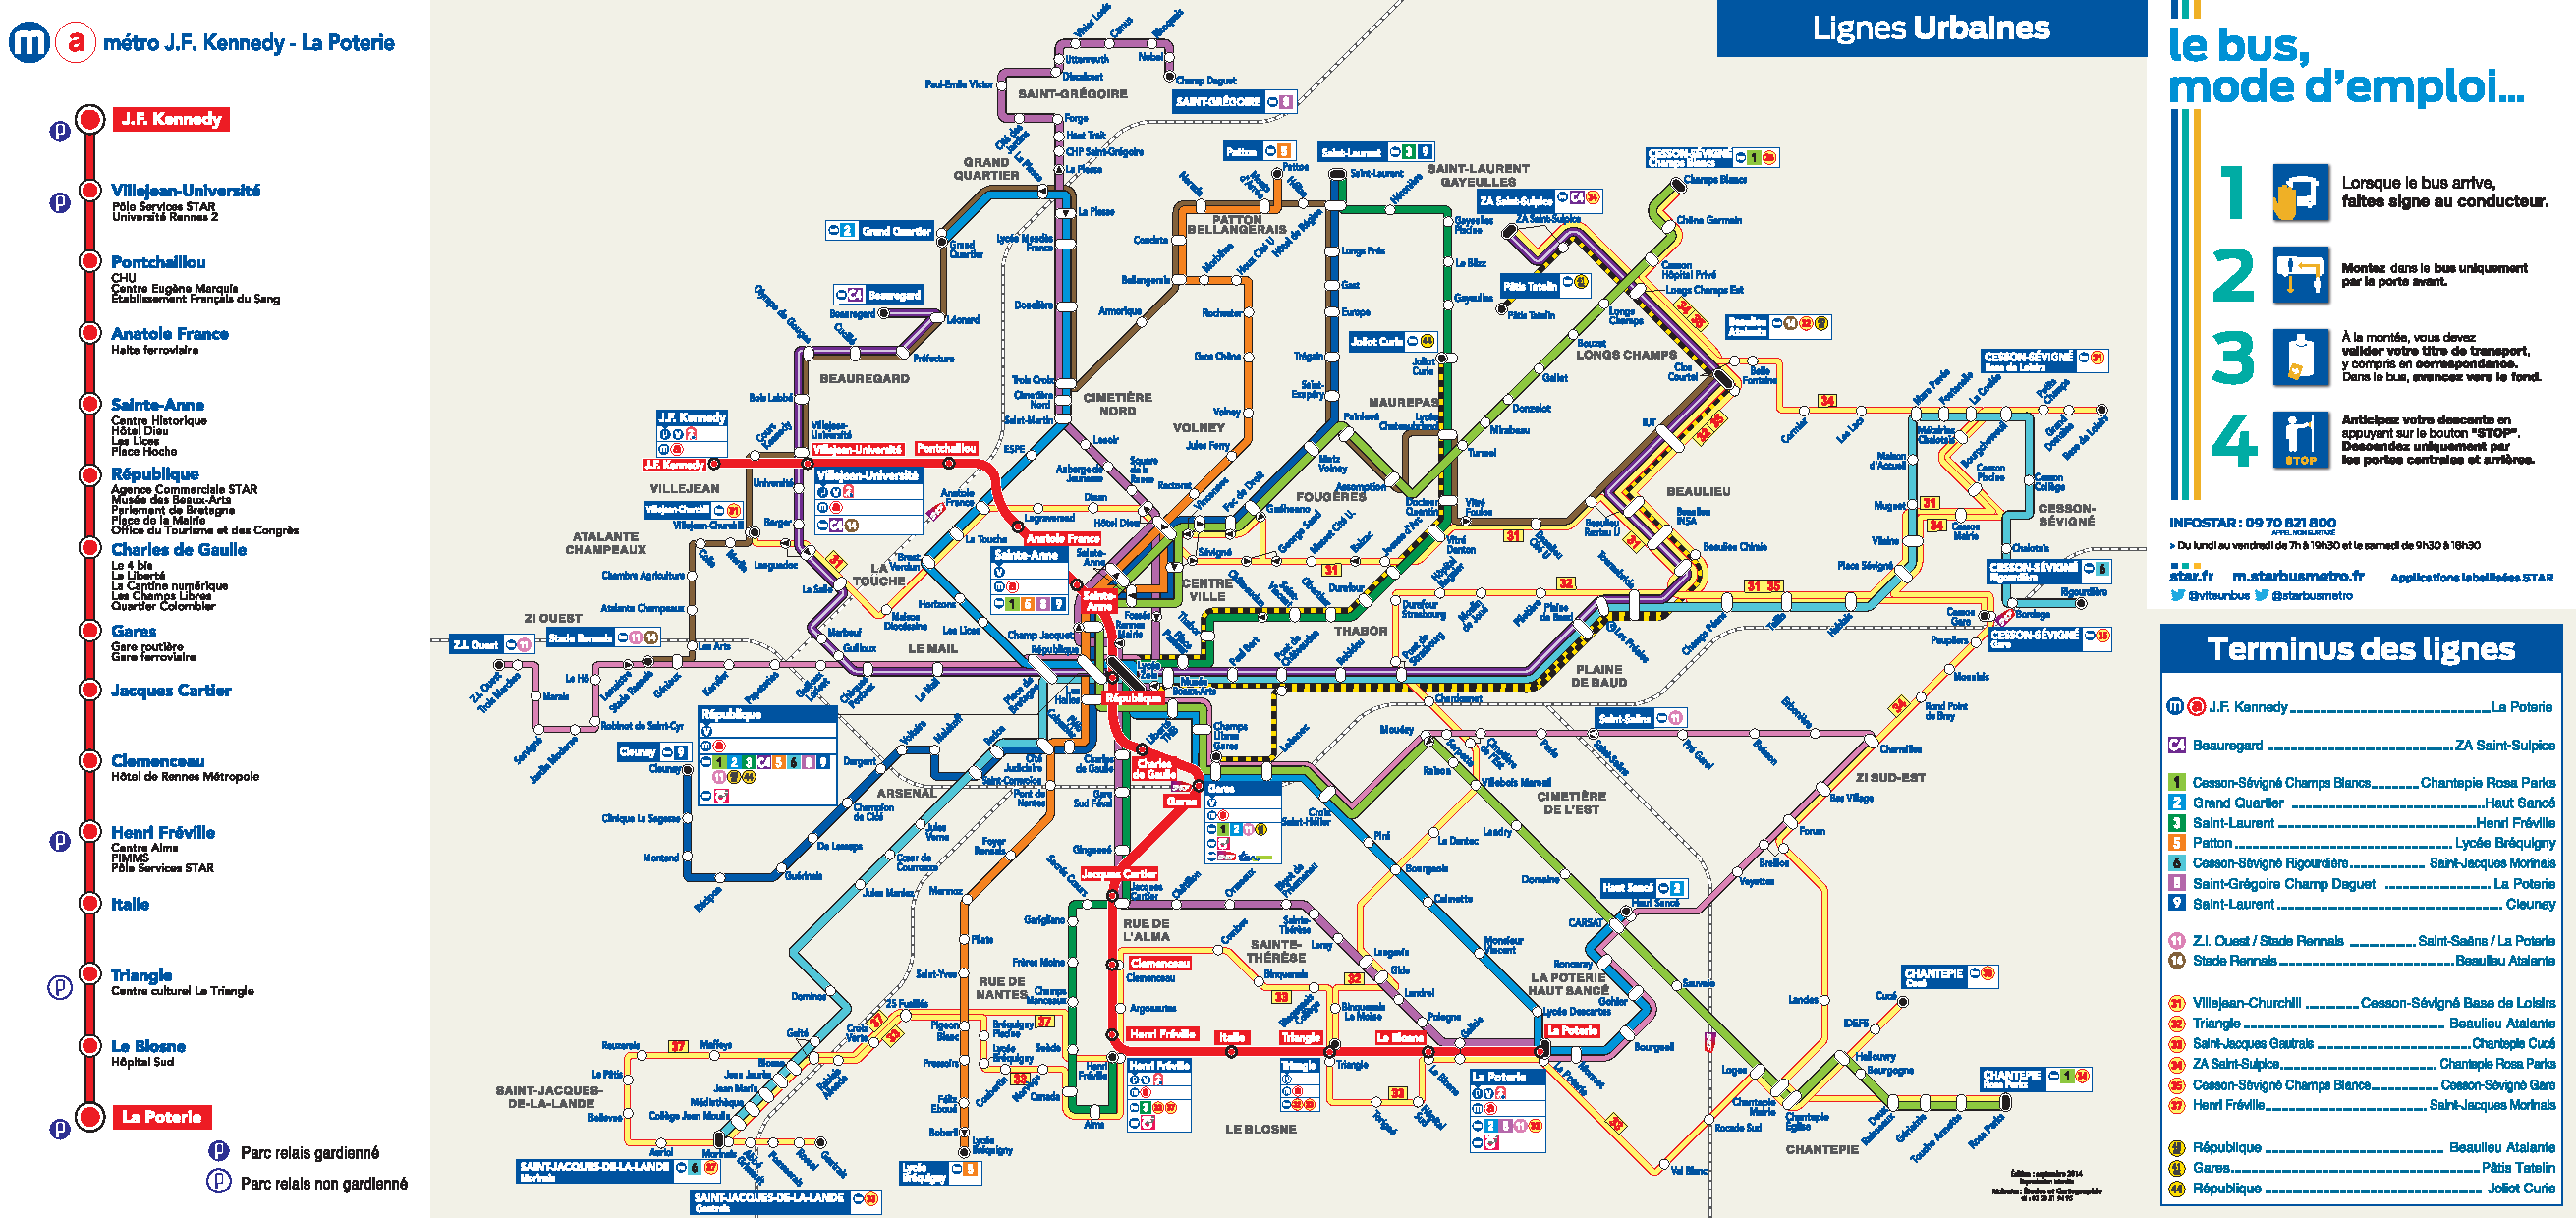
\includegraphics[width=1\textwidth]{figure/star_plan.pdf}
                \end{center}
                \caption{Le réseau du STAR est fort de vingt lignes urbaines et plus de cinquante lignes métropolitaines.}
                \label{fig:star_plan}
            \end{figure}
                
            L'information aux voyageurs passe par 870 écrans dans les bus, 70 dans les stations de métro et 50 bornes d’informations voyageurs (BIV) dans les abribus. Le système d’aide à l’exploitation et à l’information des voyageurs (SAEIV) permet d’indiquer en temps réel le passage du prochain bus, les perturbations, les correspondances, la disponibilité des vélos STAR… Ces données sont disponibles en open data, et consultables via un service mobile mis à disposition par le STAR.

            Toute cette organisation n'est cependant pas à l'abri des incidents et présente quelques failles : voici un récapitulatif des paralysies les plus importantes que nous avons trouvées.

            En juillet 2009, la ligne de métro a été bloquée pendant près de vingt heures à la suite d'un violent orage provoquant l'inondation des voies de circulation. Ceci n'est certes pas une attaque volontaire mais cela reste une faiblesse du système qu'il nous a paru intéressant de relever. 

            C'est ensuite en avril 2012 que le réseau STAR entier a été paralysé, en pleine heure de pointe, suite à l'agression d'un chauffeur. À l'époque, la direction recensait 18 agressions depuis le début de l'année, et promettait un redéploiement de ses agents de médiation et de prévention. Une mesure insuffisante pour la Confédération Française Démocratique du Travail (CFDT), qui réclamait "une police dédiée aux transports".

            Environ un mois plus tard, en mai, la ligne de métro a été entièrement bloquée (dès 5h30) pendant toute une matinée. Des bus relais ont été mis en place pour desservir les stations, jusqu'à ce que la circulation du métro reprenne (vers 14h). Selon le STAR, il s’agirait d’un problème informatique entre le centre de commandement du métro et les rames : la liaison qui permet de contrôler les rames à distance ne fonctionnait plus. Un service de bus a été mis en place pour limiter les conséquences.

            Ces quelques faits montrent bien l'importance pour le STAR de la mise en place d'un outil d'évaluation des risques, qui comporterait également un répertoire de défenses à utiliser pour contrer ces derniers.